\chapter{Requests, Web Scraping, and BS4}
As we begin to work with Pandas and data, so will the need to scrape data emerge. \newterm[Data scraping]{data scraping} is the act of pulling data off of a webpage without having to manually copy that data over. Instead, scraping data allows you to automate the process for a relatively low investment. Since you are now familiar with Pandas, you can use the full power of its data structures, plus the power of Beautiful Soup to scrape webpages efficiently.\par

\section{Webpage Structure}
To understand how we can extract data out of a webpage using web scraping, we first must understand how to read a webpage and how it is constructed. Webpages are much more than the rendered version that you see when you click on a link or navigate to a website. Webpages are actually another type of code called \newterm[HTML]{HTML}, or HyperText Markup Language. HTML is not a \textit{programming} language persay, since it does not support any of the features of a high- or low-level language. Instead, it is considered a markup language, which uses textual elements to dictate how something should be rendered by a web renderer. A HTML renderer is equivalent to the Python interpreter: it takes the code that you write and turns it into a pretty rendering. However, you can still refer to HTML as \textit{code} or as \textit{markup code}. How HTML is rendered is not dissimilar to how you can use markdown language in your \index{Jupyter Notebooks}.\par
Webpages can be constructed in several different ways, depending on the developer. However, most of the data that you will be scraping comes from HTML tables, and this is what we will focus on in this textbook.\par

\subsection{HTML}
The most obvious part of \index{HTML} is its nested nature. Objects in HTML are nested inside of larger objects, and these larger objects can dictate how a sub-object is rendered. HTML describes the structure of pages using this nesting concept.

\begin{lstlisting}[style=HTML]
<html>
    <head>
        <title>My Webpage</title>
    </head>
    <body>
        <h1>Star Wars</h1>
        <h2>Episode 4</h2>
        <p>Did you hear that? They've shut down the main reactor. We'll be destroyed for sure. This is madness! We're doomed! There'll be no escape for the Princess this time. What's that? Artoo! Artoo-Detoo, where are you? At last! Where have you been? They're heading in this direction.</p>
        <p>I want her alive! There she is! Set for stun! She'll be all right. Inform Lord Vader we have a prisoner. Hey, you're not permitted in there. It's restricted.</p>
        <p>The circle is now complete. When I left you, I was but the learner, now I am the master. Only a master of evil, Darth. Your powers are weak, old man.</p>
        <h2>Episode 6</h2>
        <p>Command station, this is ST 321. Code Clearance Blue. We're starting our approach. Deactivate the security shield. The security deflector shield will be deactivated when we have confirmation of your code transmission. Stand by...</p>
        <p>Let's go back and tell Master Luke. Tee chuta hhat yudd! Goodness gracious me! Artoo Detoowha bo Seethreepiowha ey toota odd mischka Jabba du Hutt. I don't think they're going to let us in, Artoo. We'd better go.</p>
        <p>Do they have a code clearance? It's an older code, sir, but it checks out. I was about to clear them. Shall I hold them? No. Leave them to me. I will deal with them myself. As you wish, my lord.</p>
    </body>
</html>
\end{lstlisting}

In the above markup code, take a look at the tags, written in blue. The tags include things like \verb|<p>| and \verb|<body>|. Notice how all of the tags start with a \verb|<| and end with a \verb|>|. Also observe how every tag that is created has a corresponding tag at the end. This is called a closing tag, and it can be distinguished because the first character after the opening left angle bracket \verb|<| is a forward slash: \verb|</body>|, \verb|</p>|, and \verb|</h3>|. All of the text is shown in black.\par
The above code renders to the following:

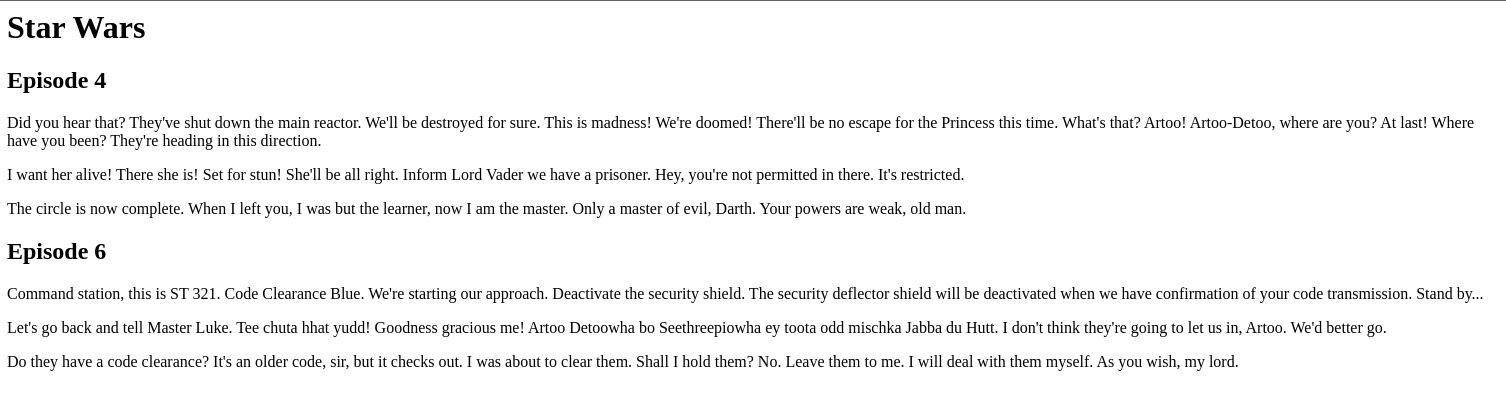
\includegraphics[width=0.8\textwidth]{img/starwarshtml.png}

Elements are usually made up of two tags: an opening tag and a closing tag. Each tag tells the renderer something about the information that sits between each of the tags. You can think of a tag like a container. The material that falls between the opening tag and the closing tag is put inside of the container that the tag created, and it is rendered according to the rules that the tag dictates.\par
Some common tags include:\par
\vspace{5mm}
\begin{tabular}{|l|l|l|}
\hline
Tag & Description              \\
\hline
\verb|<html>| & Encloses the entire HTML document \\
\hline
\verb|<head>| & Encloses special document details \\
\hline
\verb|<body>|  & Encloses the actual rendered document \\
\hline
\verb|<h1>| through \verb|<h6>| & Headers 1 through 6 \\
\hline
\verb|<i>| & Italicize \\
\hline
\verb|<b>| & Bold \\
\hline
\verb|<a>| & Hyperlink \\
\hline
\verb|<img>| & Image \\
\hline
\verb|<ul>| & Unordered (bullet pointed) List \\
\hline
\verb|<ol>| & Ordered (numbered) List \\
\hline
\verb|<li>| & List element \\
\hline
\verb|<table>| & Encloses a table's contents \\
\hline
\verb|<thead>| & Encloses a table header \\
\hline
\verb|<tbody>| & Encloses a table body \\
\hline
\verb|<tr>| & Table row \\
\hline
\verb|<td>| & Table data, or one cell in a table \\
\hline
\end{tabular}\par
\vspace{5mm}
Not all elements have two tags, and that's okay. However, these are special cases. For example, the \verb|<input>| and \verb|<br>| elements only have one tag: their opening tag. This is because all of the information that is needed to render the tag are included in the tag's \newterm[attributes]{HTML!attributes}. HTML tag attributes give additional information to the renderer about how the tag should be rendered, what the tag is, and if there's any data that needs to be dealt with. Attributes can be placed on any element, regardless of whether the tag has a closing tag or not, but they can only be placed on \textit{opening} tags, never on \textit{closing} tags.\par
There are some common attributes, including \verb|id|, \verb|class|, and \verb|name|. However, as you can see in the above HTML code snip, you don't strictly \textit{need} to include any attributes.

\subsection{CSS and JavaScript}
This is not a web design course, but it is important to understand how we get from the very simple HTML documents presented above to the websites of today.\par
CSS stands for Cascading Style Sheets, and it is responsible for styling the webpage. By providing specific rules on the size, color, shape, and placement of different elements, it is possible to create pretty webpages. Essentially, it's like putting a Snapchat filter on your boring HTML code. The HTML code provides the \textit{substance}, and the CSS provides the \textit{style}.\par
CSS can be placed in several ways: inline, in the document, or in a dedicated style sheet. If there are conflicting rules, the renderer should look at inline CSS first, then document CSS, then at the dedicated style sheet.\par
Inline styles are put in the HTML attribute \verb|style=|. Inside of the style attribute, you can write CSS code that will apply \textit{only} to the element that the styling is written on, as well as any subelements. For example, if you applied a style attribute to a \verb|div|, which typically acts as a container to enclose other elements, the style attributes on that \verb|div| would trickle down to everything inside of it. However, if that \verb|div| were inside of another \verb|div|, it would only apply to the inside \verb|div|, not the parent.\par
\boxtext{Minification}{When you write inline CSS, you are doing something called "minification". Unlike Python, CSS doesn't rely on new lines to tell when one statement has ended and another has begun. Instead, it uses semicolons. So you can just stack a bunch of style rules next to each other, separated by semicolons.}
Document CSS is written at the beginning or in the middle of an HTML document (in HTML5). Document CSS only applies to the document that the CSS is written in, but it applies to the entire document. Document CSS is placed inside of special \verb|<style></style>| tags, and it resembles what might be placed in a dedicated CSS document. In our actual document, we refer to the rules that we wrote in our \verb|<style>| tags using another HTML attribute: \verb|class=|.\par
\warningtext{Not all classes are created equal}{Classes in HTML are very different from classes in Python! Be careful to not confuse the two.}
In CSS, every group of rules is placed inside of a CSS class, which can be applied to HTML elements using the \verb|class| attribute. If all of the elements on your page are styled in a similar way, it might be possible to select what you need using the \verb|class| attribute.

\subsection{The requests Library}
In order to get the HTML into Python, we need to use a special library that can make a web request to a web server. The web server responds with what has been requested. In fact, whenever you use a website in a standard web browser, you are making requests whenever you click. There are two types of requests that are of concern to us: \verb|POST| and \verb|GET| requests.\par
POST requests are used to send data to a remote server. If you imagine a web server as a bulletin board, a POST request is asking for permission to put something on the bulletin board. The web server might deny the request, but at the very least, it must acknowledge that it received the request.\par
GET requests, as their name suggests, get data from a remote server. In our bulletin board analogy, it's equivalent to asking someone to read a listing on a bulletin board out loud to you. Again, the web server might deny the request, but it must acknowledge that you asked to get data.\par
\warningtext{Common pitfall: authentication}{Some websites require authentication. Whether this is through an username-password combination or an authentication token, this should be checked if you're having issues getting or posting data. A basic test to see if authentication is required is to just open a new Incognito, InPrivate, or Private window in a web browser, then try to directly access the resource by pasting its URL into the address bar.}
With that, it might seem like we'd only want to use GET requests. However, the inner workings of modern web frameworks are much more complicated, and they often involve asking for specific amounts of data. It's a negotiated process: you might ask for the format of the data, the web server responds with the format, you then ask if you need permissions and the web server responds with a yes, so you send the authentication token and the web server asks you what data you want, you finally send a request for what you want and the web server responds with the data. In this highly simplified scenario, we've already placed eight requests. Modern webpages might involve dozens of requests!\par
The \verb|requests| library abstracts all of this for us. We don't need to know all of the details of which requests to place and what kind of data to expect in response, since \verb|requests| already does this for us.
\subsection{Parsing with Beautiful Soup}
Now that we have our HTML in Python, we need to know how to break it apart. We could break the structure apart in a naive method, by writing a series of \verb|if| statements and iterating over the contents of the HTML until we find tags. However, why would we do this when we can use Beautiful Soup instead?\par
Beautiful Soup's job is to break apart and parse webpages in a way that is easy for you to understand. As opposed to creating a parser and writing if/else statements, Beautiful Soup comes with many tools that are incredibly powerful. The power of Beautiful Soup lies in its ability to pull data out of extraordinarily complex webpages in just a few lines of code.\par
\subsection{APIs}
An \newterm[application programming interface]{application programming interface}, or \newterm[API]{application programming interface!API}, returns formatted data based on a request that is made to it. While on the surface, an API call looks like any other web resource call, its return is very different, typically an XML or JSON form. You can experiment with open APIs using an API testing tool, like Postman. Postman can also help you form authentication strings, if your API of choice requires authentication.\par
If an API will give you the information you need, use this instead, since it's much faster to develop for.\par
There is an API for everything, and many of these APIs are free (though some still require you to get a free authentication key)! Here, we'll look at \index{application programming interface!Animechan}Animechan, an API that returns a random quote from a list of animes. Animechan doesn't require any authentication, so we can simply make a request to \href{https://animechan.vercel.app/api/random}{https://animechan.vercel.app/api/random}. If you were to just type this into a web browser, you'd get a response in the form of JSON, which can be parsed using the JSON library in Python. We'll cover this in the next section.\par

\subsection{Reading a JSON response}
Consider the Animechan API in the previous section. Let's make an example request. Based on the API documentation, we know that the API returns data in JSON form, so we can expect this in our response.
\begin{lstlisting}[style=pippython]
import requests
response = requests.get("https://animechan.vercel.app/api/random").json()
print(response)
\end{lstlisting}
Here's an example response (responses are random, but you should get a response with the same form).
\begin{lstlisting}[style=none]
{"anime":"Naruto","character":"Kiba Inuzuka","quote":"Akamaru, what's wrong boy? Have you forgotten my scent? We've always been together haven't we? We grew up together. Akamaru please, somewhere in there, there has to be a part of you that remembers. Show me that you remember. AKAMARU! Forgive me. Can you? I know that I've brought you nothing but pain and suffering. I broke my word. I swore I'd always protect you. Akamaru I'm sorry. Sorry I wasn't a better master. I'm here. Here for you. Forever."}
\end{lstlisting}
By default, the \verb|requests.get()| method returns an object of type Response, which isn't terribly useful to us on its own.\par
Observe in the request how we added the \verb|.json()| method to the end of the \verb|requests.get()| statement. Again, because we know that the API returns its data as a JSON object, we can just tell Python that we want to automatically typecast the data into a Python dictionary. The requests library will process the response as a JSON and parse it into a Python dictionary. This saves us a step down the line, explicitly parsing a JSON string into a Python dictionary. However, we still included this as an option below, since sometimes, JSON string parsing using the requests library doesn't work as we might expect.\par
We printed the data in its dictionary form, hence why we got the curly braces, keys, and values. Just like with any other Python dictionary, we can use all of our regular methods on dictionaries on this one. In our case, the dictionary is stored in a variable \verb|response|.
\begin{lstlisting}[style=pippython]
print(response["anime"])
print(response["character"])
\end{lstlisting}
\begin{lstlisting}[style=none]
Naruto
Kiba Inuzuka
\end{lstlisting}

\subsection{Parsing JSON}
This is in a form called JSON, or JavaScript Object Notation. It looks similar to a Python dictionary, and it also supports nesting. In fact, if you were to bring this into your Python script as a JSON-formatted string, you could easily parse it into a Python dictionary using the json library.\par
The json library allows us to typecast JSON data into a list or dictionary, depending whether the JSON object has keys or not. If the JSON object doesn't have any keys, then the json library will typecast the object into a Python list with an auto-assigned index. If the JSON object does have keys, like our Animechan response, then the json library will typecast the object into a Python dictionary using the keys and values from the JSON object.\par
To do this typecasting, we can use the \verb|load()| or \verb|loads()| method. They are different in the type of object they are expecting. For our purposes, we will almost always use the \verb|loads()| method. The \verb|s| in \verb|loads()| stands for string, and this particular method is used to parse a string containing JSON data into a Python dictionary or list.\par
Let's make another request, but this time, let's specify that we want the string form of the data, rather than letting the requests library parse the JSON object for us. As we did when we were getting the contents of the HTML webpage, we can specify this by specifying that we want the \verb|text| attribute from the \verb|response| object.
\begin{lstlisting}[style=pippython]
response = requests.get("https://animechan.vercel.app/api/random").text
print(type(response))
print(response)
\end{lstlisting}
\begin{lstlisting}[style=none]
str
{"anime":"Death Note","character":"Light Yagami","quote":"This is the first time in my life that I've been provoked to hit a woman."}
\end{lstlisting}
This time, our response is left in the string form that it was given to us by the API. We can parse this using the \verb|loads()| method in the json library. \verb|loads()| typically only takes one argument, the string with the JSON-formatted string.
\begin{lstlisting}[style=pippython]
response = json.loads(response)
print(type(response))
print(response)
\end{lstlisting}
\begin{lstlisting}[style=none]
<class 'dict'>
{'anime': 'Death Note', 'character': 'Light Yagami', 'quote': "This is the first time in my life that I've been provoked to hit a woman."}
\end{lstlisting}
We can now see that the type is no longer \verb|str| but is a dictionary object instead.\par
The key with the \verb|load()| and \verb|loads()| methods is that they work on any JSON-formatted data, not just data that comes from a web request. For example, consider if we imported a JSON as a file and read it into a string variable, as we showed in Chapter 8. We could then use the \verb|loads()| method to parse this string into a Python dictionary.